
\hzsync{equation}{56}
\hzsync{theorem}{5}

\section{\trConvex\trEnergySurface{}上\trPeriodicOrbit{}的存在性}
\label{sec:periodic-orbit-convex}

本节我们将证明一个非常特殊的定性存在性结果，它在历史上标志着%
\trSymplecticGeometry{}与\textbf{\trHamiltonian{}力学}（Hamiltonian mechanics）%
的整体性问题快速发展的开端。我们的目的在于展示\trCalculusOfVariations{}之%
\trDirectMethod{}这一经典技巧。该技巧与第 3 章中引入的较新技巧恰成鲜明对照。%
在第 4 章中，这个结果本身将是某个特殊\trSymplecticInvariant{}之存在性的直接推论。

\begin{theorem}\label{thm:convex-closed-orbit}
设\trHypersurface{} $S\subset(\R^{2n},\omega_{0})$ 是 $\R^{2n}$ 中一个%
\trCompact{}且\trStrictlyConvex{}的\textbf{\trDomain}（region）的\trSmooth{}%
（属于 $C^{2}$ 类的）\trBoundary。则 $S$ 带有一条\trClosed\trOrbit。
\end{theorem}

特别地，我们得出：凡以 $S$ 为一个\trRegular\trEnergySurface{}的%
\trHamiltonianVectorField{} $X_{H}$ 都在 $S$ 上具有\trPeriodicSolution。%
该结果归于 P.~\trRabinowitz{}[180] 与 A.~\trWeinstein{}[225]（1978）。%
我们下面给出的证明基于 F.~\trClarke{}[53] 的一个想法。

\begin{proof}
为证明该定理，我们利用选取便利的\trHamiltonianFunction{}这一自由，%
并引入一个特定的\trHamiltonianFunction{} $H$——它是次数为 $2$ 的正\trHomogeneous{}函数——%
并把该\trHypersurface{}表示为 $S=\{x\in\R^{2n}\mid H(x)=1\}$。%
$S$ 是 $\R^{2n}$ 中一个\trCompact{}且\trStrictlyConvex{}的\trDomain{} $C$ 的%
\trBoundary，我们可以假定 $C$ 在其\textbf{\trInterior}（interior）中包含原点。%
于是，从原点出发的每一条射线都非切向地与 $S$ 恰好交于一点。%
因此，若给定 $x\neq0$，则在 $S$ 上存在唯一一点 $\xi=\lambda^{-1}x$，其中 $\lambda>0$。

\noindent\begin{minipage}{\linewidth}
\centering
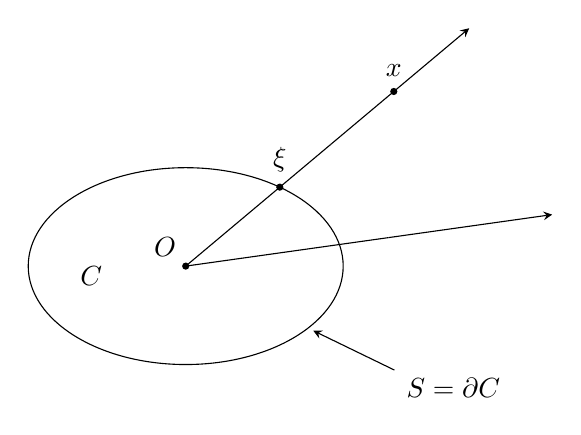
\begin{tikzpicture}[>=stealth]
  \draw (0,0) ellipse (2 and 1.25);%
  \fill (0,0) circle (1.3pt) node[above left] {$O$};
  \node at (-1.2,-0.12) {$C$};
  \draw (0,0) -- (40:2.4);%
  \draw[->] (40:2.4) -- (40:4.7);
  \fill (40:1.56) circle (1.3pt) node[above=2pt] {$\xi$};%
  \fill (40:3.45) circle (1.3pt) node[above=2pt] {$x$};
  \draw (0,0) -- (8:2.6);%
  \draw[->] (8:2.6) -- (8:4.7);
  \node at (3.4,-1.55) {$S=\partial C$};
  \draw[->] (2.65,-1.32) -- (1.62,-0.82);%
\end{tikzpicture}

图 1.2
\end{minipage}

若在 $\R^{2n}$ 上如下定义函数 $F$：当 $x\neq0$ 时，取 $\xi=\lambda^{-1}x\in S$%
并令 $F(x)=\lambda$；再令 $F(0)=0$——那么\trManifold{} $S$ 便可表示为%
$S=\{x\mid F(x)=1\}$。我们希望借助一个\trStrictlyConvex{}的函数 $H$%
把 $S$ 描述为\trLevelSet{}$\{x\mid H(x)=1\}$，也就是说，要求 $H$ 的%
\trHessian{} $H_{xx}(x)$ 在每个点 $x\neq0$ 处都\trPositiveDefinite。%
由于 $F$ 是一次\trHomogeneous{}的，它显然绝不\trStrictlyConvex。事实上，%
对\trEuler{}公式 $\langle F_{x},x\rangle=F$ 求导便给出 $F_{xx}x=0$。%
按\textbf{\trConvexity}（convexity）假设，$F_{xx}\big|_{TS}>0$。于是我们定义函数
\[
H(x)=\bigl(F(x)\bigr)^{2}
\]
它恰在 $S$ \trStrictlyConvex{}时才\trStrictlyConvex，这一点不难证明。%
我们于是便证明了：每个在其\trInterior{}中包含原点的\trStrictlyConvex\trEnergySurface{} $S$%
都可以表示为
\begin{equation}\label{eq:s-level-set}
S\ =\ \bigl\{\,x\ \bigm|\ H(x)=1\,\bigr\}
\end{equation}
其中的函数 $H:\R^{2n}\longrightarrow\R$ 满足
\begin{equation}\label{eq:h-properties}
\begin{array}{lll}
\text{(i)}   &\ H\in C^{2}(\R^{2n}\backslash\{0\}), &\ H(0)=0\\[4pt]
\text{(ii)}  &\ H_{xx}(x)>0 &\ \text{若}\quad x\neq0\\[4pt]
\text{(iii)} &\ H(\rho x)=\rho^{2}H(x) &\ \text{若}\quad \rho\geq0.
\end{array}
\end{equation}

鉴于我们在上一节中的讨论，只需证明：这个特定的\trHamiltonianVectorField{} $X_{H}$%
在该\trEnergySurface{} $S$ 上具有\trPeriodicSolution，也就是说，%
我们必须证明：在 $S$ 上存在
\[
\dot{x}=J\nabla H(x)
\]
的\trPeriodicSolution。把\trPeriodic{}规范化后，我们便可以在 $S$ 上寻求%
\trPeriodic{}为 $2\pi$ 的、如下方程的\trPeriodicSolution：
\begin{equation}\label{eq:normalized-equation}
\dot{x}=\lambda\,J\nabla H(x)\qquad\text{对某个}\quad\lambda\neq0.
\end{equation}
例如，\trVariationalPrinciple
\[
\min\int_{0}^{2\pi}H\bigl(x(t)\bigr)\,dt\qquad\text{约束于}\quad
\frac{1}{2}\int_{0}^{2\pi}\langle Jx,\dot{x}\rangle=1\,,
\]
（其中诸函数 $x(t)$ 均假定\trPeriodic{}为 $2\pi$）就以上述方程为其\trEuler{}方程。%
但容易证明：即使在 $H(x)=\frac{1}{2}|x|^{2}$ 的情形，下确界与上确界也都不被取到。%
现在的技巧在于改用另一个\trVariationalPrinciple，它具有同样的\trDifferentialEquation，%
但其下确界却被取到。我们将对 $H$ 作\trLegendre{}变换；但与物理学中通常的\trLegendre{}变换不同，%
这里一切变量都将被变换。由\trLegendre{}变换与 $H(x)$ 相联系的函数 $G(y)$ 可定义为
\[
G(y)=\max_{\xi\in\R^{2n}}\Bigl(\langle\xi,y\rangle-H(\xi)\Bigr)=\langle x,y\rangle-H(x).
\]
的确存在唯一的最大值点 $x\in\R^{2n}$，它由 $y=\nabla H(x)$ 给出；%
这是因为 $H_{xx}(y)$ 在 $y\neq0$ 时\trPositiveDefinite，而且 $H$ 满足
\begin{equation}\label{eq:h-quadratic-estimate}
\frac{1}{c}\,|y|^{2}\leq H(y)\leq c\,|y|^{2},\qquad y\in\R^{2n}
\end{equation}
其中常数 $c>1$。该\textbf{\trEstimate}（estimate）是 $H$ 的\textbf{\trHomogeneity}%
（homogeneity）的直接推论。总括起来，我们有
\begin{equation}\label{eq:legendre-identity}
G(y)+H(x)=\langle x,y\rangle
\end{equation}
其中
\begin{equation}\label{eq:gradient-inverse}
y=\nabla H(x)\qquad\text{且}\qquad x=\nabla G(y).
\end{equation}
显然 $G(0)=0$，$G\in C^{2}(\R^{2n}\backslash\{0\})$，并且 $G$ 是二次正\trHomogeneous{}的。%
由于当 $x\neq0$ 时 $H_{xx}(x)\cdot G_{yy}(y)=\mathbf{1}$，故当 $y\neq0$ 时%
$G$ 也\trStrictlyConvex，从而 $G$ 具有与 $H$ 相同的性质：
\[
\begin{array}{ll}
\text{(i)}   &\ G(0)=0,\ G\in C^{2}(\R^{2n}\backslash\{0\})\\[4pt]
\text{(ii)}  &\ G_{yy}(y)>0\qquad\text{若}\quad y\neq0\\[4pt]
\text{(iii)} &\ G(\rho y)=\rho^{2}G(y)\qquad\text{对}\quad \rho\geq0.
\end{array}
\]

现在，我们来看针对\trPeriodic{}为 $2\pi$ 的函数 $z$ 的这个新的替代性%
\trVariationalPrinciple：
\begin{equation}\label{eq:alternate-principle}
\min\int_{0}^{2\pi}G(\dot{z})\,dt\qquad\text{约束于}\quad
\frac{1}{2}\int_{0}^{2\pi}\langle Jz,\dot{z}\rangle=1\,,
\end{equation}
我们将以\trStandard{}的直接变分方法求解它。更精确地说，我们定义如下由%
平均值为 $0$ 的\trPeriodic{}函数 $z(t)=z(t+2\pi)$ 组成的函数空间 $\mathcal{F}$：
\[
\mathcal{F}=\Bigl\{\,z\in H_{1}(S^{1})\ \Bigm|\ \frac{1}{2\pi}\int_{0}^{2\pi}z(t)\,dt=0\,\Bigr\}\,,
\]
其中 $H_{1}(S^{1})$ 是由绝对连续且\trPeriodic{}为 $2\pi$ 的函数组成的%
\trHilbert{}空间，这些函数的\trDerivative{}都是平方可积的，即属于 $L_{2}(S^{1})$。%
注意，与 $z$ 一起，$z+\mathrm{const.}$ 也是 \eqref{eq:alternate-principle} 的解，%
因此平均值条件恰好把这个常数固定下来。以 $\mathcal{A}\subset\mathcal{F}$ 表示子集
\[
\mathcal{A}=\Bigl\{\,z\in\mathcal{F}\ \Bigm|\ \frac{1}{2}\int_{0}^{2\pi}\langle Jz,\dot{z}\rangle=1\,\Bigr\}.
\]
按照\trStandard{}的程序，我们将验证\trFunctional
\[
I(z)=\int_{0}^{2\pi}G\bigl(\dot{z}(t)\bigr)\,dt\qquad\text{于}\quad\mathcal{A}
\]
满足以下诸性质：
\begin{enumerate}[label=(\roman*)]
\item 它在 $\mathcal{A}$ 上是\trBoundedBelow{}的。
\item 它在 $\mathcal{A}$ 上取到最小值，即存在 $z_{*}\in\mathcal{A}$ 满足
\[
\int_{0}^{2\pi}G(\dot{z}_{*})\,dt=\inf_{z\in\mathcal{A}}\int_{0}^{2\pi}G(\dot{z})\,dt=\mu>0.
\]
\item $z_{*}$ 求解\trEuler{}方程
\[
\nabla G(\dot{z}_{*})=\alpha Jz_{*}+\beta
\]
（在 $L^{2}(S^{1})$ 中），其中 $\alpha\neq0$ 与 $\beta$ 为常数。
\item $z_{*}$ 属于 $C^{2}$，且逐点满足
\[
\dot{z}_{*}=\nabla H(\alpha Jz_{*}+\beta)
\]
而 $x(t)=c\,\bigl(\alpha Jz_{*}(t)+\beta\bigr)$ 便是所要的解，%
即 $\dot{x}=J\nabla H(x)$ 在 $S$ 上对适当常数 $c$ 的解。
\end{enumerate}

\medskip
\noindent\emph{关于（i）：}我们需要一些\trEstimate。%
由于属于 $\mathcal{F}$ 的每个 $z$ 的平均值都为零，\trPoincare{}不等式
\[
\|z\|\leq\|\dot{z}\|\,,\qquad z\in\mathcal{F}
\]
成立，其中 $\|\cdot\|$ 表示 $L_{2}$ \textbf{\trNorm}（norm）。%
这由\trFourier{}级数即可得证。对 $z\in\mathcal{A}$ 我们得出
\begin{equation}\label{eq:poincare-consequence}
2=\int_{0}^{2\pi}\langle Jz,\dot{z}\rangle\ \leq\ \|z\|\,\|\dot{z}\|\ \leq\ \|\dot{z}\|^{2},\qquad z\in\mathcal{A}.
\end{equation}
函数 $G$ 因其\trStrictlyConvex{}且二次正\trHomogeneous，满足\trEstimate{}%
$\frac{1}{K}|y|^{2}\leq G(y)\leq K|y|^{2}$（$y\in\R^{2n}$），其中常数 $K\geq1$。%
于是，借助 \eqref{eq:poincare-consequence}，对 $z\in\mathcal{A}$ 我们得到
\begin{equation}\label{eq:functional-lower-bound}
\int_{0}^{2\pi}G(\dot{z})\,dt\ \geq\ \frac{1}{K}\|\dot{z}\|^{2}\ \geq\ \frac{2}{K}>0\,,
\end{equation}
也就是说，该\trFunctional{}以一个正常数为下界；特别地，$\mu>0$。

\medskip
\noindent\emph{关于（ii）：}我们选取\textbf{\trMinimizingSequence}（minimizing sequence）%
$z_{j}\in\mathcal{A}$ 使得
\begin{equation}\label{eq:minimizing-sequence}
\lim_{j\to\infty}\int_{0}^{2\pi}G(\dot{z}_{j})\,dt=\mu.
\end{equation}
鉴于 \eqref{eq:poincare-consequence} 与 \eqref{eq:functional-lower-bound}，%
存在常数 $M>0$ 使 $2\leq\|\dot{z}_{j}\|^{2}\leq M$，于是我们得到%
$\|z_{j}\|\geq2\|\dot{z}_{j}\|^{-1}\geq\frac{2}{\sqrt{M}}$，%
从而由\trPoincare{}不等式进一步得到 $\frac{2}{\sqrt{M}}\leq\|z_{j}\|\leq\sqrt{M}$。%
特别地，$z_{j}$ 是\trHilbert{}空间 $H_{1}(S^{1})$ 中的\trBounded{}序列，%
因此存在一个子序列（仍记作 $z_{j}$）在 $H_{1}(S^{1})$ 中弱收敛到某个元素%
$z_{*}\in H_{1}(S^{1})$：
\begin{equation}\label{eq:weak-convergence}
z_{j}\rightarrow z_{*}\qquad\text{在}\ H_{1}(S^{1})\ \text{中弱收敛}.
\end{equation}
这里用到了一个众所周知的事实：\trHilbert{}空间的\textbf{\trClosed\trUnitBall}%
（closed unit ball）是弱序列紧的。此外，对函数 $\hat{z}_{*}\in C(S^{1})$，
\begin{equation}\label{eq:uniform-convergence}
\sup_{t}\bigl|z_{j}(t)-\hat{z}_{*}(t)\bigr|\rightarrow0\,,
\end{equation}
即 $z_{j}$ 一致收敛到 $\hat{z}_{*}$。事实上，诸 $z_{j}$ 是等度连续的：
\begin{align*}
\bigl|z_{j}(t)-z_{j}(\tau)\bigr|\ &\leq\ \Bigl|\int_{\tau}^{t}\dot{z}_{j}(s)\,ds\Bigr|\\
&\leq\ |t-\tau|^{1/2}\,\|\dot{z}_{j}\|\\
&\leq\ |t-\tau|^{1/2}\sqrt{M}\,,
\end{align*}
而断言便由\trArzela{}--\trAscoli{}定理得出。显然 $z_{*}(t)=\hat{z}_{*}(t)$%
\trAlmostEverywhere{}成立。事实上，借助 $L^{2}$ \trInnerProduct{}我们可以写%
$\bigl(z_{*}-\hat{z}_{*},\,z_{*}-\hat{z}_{*}\bigr)=\bigl(z_{j}-\hat{z}_{*},\,z_{*}-\hat{z}_{*}\bigr)+\bigl(z_{*}-z_{j},\,z_{*}-\hat{z}_{*}\bigr)$；%
右端第一项由一致收敛趋于 $0$，第二项由弱收敛趋于 $0$。

我们将证明 $z_{*}\in\mathcal{A}$。由 \eqref{eq:uniform-convergence} 可知%
$z_{*}$ 的平均值为零。此外，
\[
2=\int_{0}^{2\pi}\langle Jz_{j},\dot{z}_{j}\rangle
 =\int_{0}^{2\pi}\bigl\langle J(z_{j}-z_{*}),\,\dot{z}_{j}\bigr\rangle
 +\int_{0}^{2\pi}\langle Jz_{*},\,\dot{z}_{j}\rangle.
\]
右端第一项由 \eqref{eq:uniform-convergence} 趋于 $0$，因为%
$\|\dot{z}_{j}\|\leq\sqrt{M}$ \trBounded；第二项由 \eqref{eq:weak-convergence} 收敛，于是
\[
\int_{0}^{2\pi}\langle Jz_{*},\ \dot{z}_{*}\rangle=2
\]
从而 $z_{*}\in\mathcal{A}$。接着我们证明这个 $z_{*}$ 是最小值点。%
由 $G$ 的\trConvexity{}我们得到逐点\trEstimate{}%
$\bigl\langle\nabla G(y_{1}),\,y_{2}-y_{1}\bigr\rangle\leq G(y_{2})-G(y_{1})\leq\bigl\langle\nabla G(y_{2}),\,y_{2}-y_{1}\bigr\rangle$，%
将其应用于 $\dot{z}_{*}(t)=y_{2}$ 与 $y_{1}=\dot{z}_{j}(t)$ 便给出
\[
\int_{0}^{2\pi}G(\dot{z}_{*})\,dt-\int_{0}^{2\pi}G(\dot{z}_{j})\,dt\ \leq\
\int_{0}^{2\pi}\bigl\langle\nabla G(\dot{z}_{*}),\ \dot{z}_{*}-\dot{z}_{j}\bigr\rangle\,dt.
\]
注意到 $\nabla G$ 作为一次正\trHomogeneous{}的\trMapping{}满足\trEstimate{}%
$|\nabla G(y)|\leq C|y|$（$y\in\R^{2n}$，$C>0$ 为某常数），%
我们便得出 $\nabla G(\dot{z}_{*})$ 属于 $L_{2}$，从而右端趋于零，%
因为 $\bigl(\dot{z}_{*}-\dot{z}_{j}\bigr)\rightarrow0$ 于 $L_{2}$ 中弱收敛。%
这样，由 \eqref{eq:minimizing-sequence} 得
\[
\mu\ \leq\ \int_{0}^{2\pi}G(\dot{z}_{*})\,dt\ \leq\
\liminf_{j\to\infty}\int_{0}^{2\pi}G(\dot{z}_{j})\,dt=\mu,
\]
我们便证明了：$z_{*}$ 是 $I(z)$ 在 $\mathcal{A}$ 上的最小值点\footnote{上式首项积分 $\int_{0}^{2\pi}G(\dot{z}_{*})$，原书漏排 $dt$，此处补齐。——译者注}。

\medskip
\noindent\emph{关于（iii）：}由于 $z_{*}$ 是最小值点，我们有
\begin{equation}\label{eq:first-variation}
\int_{0}^{2\pi}\bigl\langle\nabla G(\dot{z}_{*}),\,\dot{\zeta}\bigr\rangle=0
\end{equation}
对每个满足
\begin{equation}\label{eq:test-constraint}
\int_{0}^{2\pi}\langle Jz_{*},\,\dot{\zeta}\rangle=0
\end{equation}
的\textbf{\trTestFunction}（test function）$\zeta\in\mathcal{F}$ 成立。%
现在我们选取形如下式的 $\zeta$：
\[
\dot{\zeta}=\nabla G(\dot{z}_{*})-\alpha Jz_{*}-\beta
\]
其中 $\alpha$ 与 $\beta$ 为两个常数。为使 $\zeta$ 成为周期的，%
我们如此选取 $\beta$，使 $\dot{\zeta}$ 的平均值为零：
\[
\int_{0}^{2\pi}\dot{\zeta}\,dt=\int_{0}^{2\pi}\nabla G(\dot{z}_{*})\,dt-2\pi\beta=0\,,
\]
然后再确定常数 $\alpha$，使 \eqref{eq:test-constraint} 成立。%
再次利用 $z_{*}$ 的平均值为零这一事实，我们发现方程
\begin{equation}\label{eq:alpha-equation}
0=\int_{0}^{2\pi}\langle Jz_{*},\,\dot{\zeta}\rangle
 =\int_{0}^{2\pi}\bigl\langle Jz_{*},\,\nabla G(\dot{z}_{*})\bigr\rangle
 -\alpha\int_{0}^{2\pi}\langle Jz_{*},\,Jz_{*}\rangle
\end{equation}
有唯一解 $\alpha$，因为其系数不为零。利用这个\trTestFunction{} $\zeta$ 我们算得
\[
\int_{0}^{2\pi}|\dot{\zeta}|^{2}
 =\int_{0}^{2\pi}\bigl\langle\nabla G(\dot{z}_{*}),\,\dot{\zeta}\bigr\rangle
 -\alpha\int_{0}^{2\pi}\langle Jz_{*},\,\dot{\zeta}\rangle
 -\Bigl\langle\beta,\ \int_{0}^{2\pi}\dot{\zeta}\Bigr\rangle
\]
而由条件 \eqref{eq:first-variation} 知上式为零。我们于是得出：$z_{*}$ 满足\trEuler{}方程
\begin{equation}\label{eq:euler-equation}
\nabla G(\dot{z}_{*})=\alpha Jz_{*}+\beta
\end{equation}
其中 $\alpha$ 与 $\beta$ 为常数——这当然不出所料。对这个常数 $\alpha$%
我们求得 $\alpha=\mu$，从而 $\alpha>0$。事实上，利用\trEuler{}方程%
\eqref{eq:euler-equation} 与 $G$ 的\trHomogeneity，我们算得
\[
2\mu=2\int_{0}^{2\pi}G(\dot{z}_{*})
 =\int_{0}^{2\pi}\bigl\langle\nabla G(\dot{z}_{*}),\,\dot{z}_{*}\bigr\rangle
 =\alpha\int_{0}^{2\pi}\langle Jz_{*},\,\dot{z}_{*}\rangle=2\alpha\,.
\]

\medskip
\noindent\emph{关于（iv）：}容易看出 $z_{*}$ 属于 $C^{2}$。%
回忆 $x=\nabla G(y)$ 由 $y=\nabla H(x)$ 逐点求逆，我们便从\trEuler{}方程得到
\begin{equation}\label{eq:zstar-h}
\dot{z}_{*}(t)=\nabla H\bigl(\alpha Jz_{*}(t)+\beta\bigr)
\end{equation}
对\trAlmostEvery{}的 $t$ 成立。上式右端是连续的，于是我们得出 $z_{*}\in C^{1}$；%
再把它代回右端，便发现 $z_{*}\in C^{2}$。最后，令
\[
x(t)=c\,\Bigl(\alpha Jz_{*}(t)+\beta\Bigr),
\]
其中 $c>0$，我们由 \eqref{eq:zstar-h} 并利用 $\nabla H$ 的\trHomogeneity{}得到
\[
\dot{x}=c\,\alpha J\,\nabla H\bigl(\alpha Jz_{*}+\beta\bigr)=\alpha J\,\nabla H(x)
\]
又因 $H$ 是二次\trHomogeneous{}的，
\[
\int_{0}^{2\pi}H(x)\,dt=\frac{1}{2}\int_{0}^{2\pi}\bigl\langle\nabla H(x),\,x\bigr\rangle\
 =\ \frac{1}{2}\,c^{2}\alpha\int_{0}^{2\pi}\langle\dot{z}_{*},\,Jz_{*}\rangle=c^{2}\alpha
\]
若取 $c=\sqrt{\dfrac{2\pi}{\alpha}}$，上式便等于 $2\pi$。于是，$x(t)$ 是方程%
$\dot{x}=\alpha J\,\nabla H(x)$ 的一个\trPeriodic{}为 $2\pi$ 的\trPeriodicSolution，%
并且位于\trEnergySurface{} $H=1$ 之上。从而，$y(t)=x\bigl(\alpha^{-1}t\bigr)$%
便是所要的、$\dot{x}=J\nabla H(x)$ 在 $H=1$ 上的\trPeriodicSolution，%
其\trPeriodic{}为 $T=2\pi\alpha=2\pi\mu$。但这无关紧要，%
因为 $S$ 上\trPeriodicSolution{}的\trPeriodic{}取决于我们对%
\trHamiltonianFunction{}的选取。定理证毕。
\end{proof}

回忆\trHamiltonianVectorField{}的变换性质，由上述定理可以得出：%
$\R^{2n}$ 中凡与某个\trStrictlyConvex{}的\trHypersurface{}之间存在%
\trSymplecticDiffeomorphism{}的\trHypersurface，都必具有\trClosedCharacteristic。%
然而，这种情形很难辨认；我们在下文将会看到，确有与\trConvex\trHypersurface{}之间不存在%
\trSymplecticDiffeomorphism{}的\trHypersurface。我们在第 4 章中的目标，%
将是描述\trHypersurface{}在辛意义下\trInvariant{}的、保证\trClosedCharacteristic{}%
存在性的那些性质。不过，这一存在性将由一个颇为不同的\trVariationalPrinciple{}来建立。

上述证明的想法有时被称为\textbf{\trDual\trAction{}原理}（dual action principle），%
它催生了关于\textbf{\trConvex\trHamiltonianFunction}（convex Hamiltonian）的%
许多存在性结果。例如，I.~\trEkeland{}[65] 于 1984 年为\trConvex\trHypersurface{}上的%
\trPeriodicSolution{}建立了一个\trMorseTheory，它类似于\trCompact\trRiemann\trManifold{}上%
\textbf{\trClosed\trGeodesic}（closed geodesic）的相应理论。%
利用\trEkeland{}的\trMorseTheory，他证明了：在\trGeneric{}意义下%
（属于 $C^{\infty}$ 范畴），每个\trCompact{}且\trConvex{}的\trHypersurface{}%
$S\subset\R^{2n}$ 都带有无穷多条\trPeriodicOrbit{}[65, 66, 67]。%
在特殊情形，即\trConvex\trSurface{} $S\subset\R^{2n}$ 接近一个\textbf{圆\trSphere}%
（round sphere）——此时存在半径为 $r$ 与 $R$ 的两个开\trBall{}使得
\[
B(r)\subset S\subset B(R)\qquad\text{且}\qquad R\leq\sqrt{2}\,r
\]
（其中第一个包含关系意指包含于 $S$ 的\trInterior{}之中）——%
则可以证明：$S$ 至少带有 $n$ 条\trClosedCharacteristic{}[70]。%
这里的\trConvexity{}要求可以稍稍放宽，确切陈述请参见 [21]。

关于这一类涉及\trConvex\trHamiltonianFunction{}的问题的综述，%
请参见 I.~\trEkeland{}的新近专著《Convexity Methods in Hamiltonian Mechanics》%
（1990）[66]。
